\documentclass[a4paper]{article}
\usepackage{vntex}
%\usepackage[english,vietnam]{babel}
%\usepackage[utf8]{inputenc}

%\usepackage[utf8]{inputenc}
%\usepackage[francais]{babel}
\usepackage{a4wide,amssymb,epsfig,latexsym,array,hhline,fancyhdr}
\usepackage[normalem]{ulem}
%\usepackage{soul}

\usepackage[makeroom]{cancel}
\usepackage{amsmath}
\usepackage{amsthm}
\usepackage{multicol,longtable,amscd}
\usepackage{diagbox}%Make diagonal lines in tables
\usepackage{booktabs}
\usepackage{alltt}
\usepackage[framemethod=tikz]{mdframed}% For highlighting paragraph backgrounds
\usepackage{caption,subcaption}
\usepackage{hyperref}

\usepackage{lastpage}
\usepackage[lined,boxed,commentsnumbered]{algorithm2e}
\usepackage{enumerate}
\usepackage{color}
\usepackage{graphicx}							% Standard graphics package
\usepackage{array}
\usepackage{tabularx, caption}
\usepackage{multirow}
\usepackage{multicol}
\usepackage{rotating}
\usepackage{graphics}
\usepackage{geometry}
\usepackage{setspace}
\usepackage{epsfig}

\usepackage{tikz}

% \usepackage{fontspec}
\usepackage{minted}
\usetikzlibrary{arrows,snakes,backgrounds}
\usepackage[unicode]{hyperref}
\hypersetup{urlcolor=black,linkcolor=black,citecolor=black,colorlinks=true} 

%\usepackage{pstcol} 								% PSTricks with the standard color package

\usepackage[normalem]{ulem}

\newtheorem{theorem}{{\bf Định lý}}
\newtheorem{property}{{\bf Tính chất}}
\newtheorem{proposition}{{\bf Mệnh đề}}
\newtheorem{corollary}[proposition]{{\bf Hệ quả}}
\newtheorem{lemma}[proposition]{{\bf Bổ đề}}
\theoremstyle{definition}
\newtheorem{exer}{Bài toán}

\def\thesislayout{	% A4: 210 × 297
	\geometry{
		a4paper,
		total={160mm,240mm},  % fix over page
		left=30mm,
		top=30mm,
	}
}
\thesislayout
% \DeclareUnicodeCharacter{U+2223}{"|"}
%\usepackage{fancyhdr}
\setlength{\headheight}{40pt}
\pagestyle{fancy}
\fancyhead{} % clear all header fields
\fancyhead[L]{
 \begin{tabular}{rl}
    \begin{picture}(25,15)(0,0)
    \put(0,-8){
\includegraphics[width=8mm, height=8mm]{Images/uet.png}}
    %\put(0,-8){\epsfig{width=10mm,figure=hcmut.eps}}
   \end{picture}&
	%\includegraphics[width=8mm, height=8mm]{hcmut.png} & %
	\begin{tabular}{l}
		\textbf{\bf \ttfamily Trường đại học Công nghệ}\\
		\textbf{\bf \ttfamily Đại học Quốc gia Hà Nội}
	\end{tabular} 	
 \end{tabular}
}
\fancyhead[R]{
	\begin{tabular}{l}
		\tiny \bf \\
		\tiny \bf 
	\end{tabular}  }
\fancyfoot{} % clear all footer fields
\fancyfoot[L]{\scriptsize \ttfamily Các vấn đề hiện đại trong CNTT INT3507\_6}
\fancyfoot[R]{\scriptsize \ttfamily Trang {\thepage}/\pageref{LastPage}}
\renewcommand{\headrulewidth}{0.3pt}
\renewcommand{\footrulewidth}{0.3pt}


%%%
\setcounter{secnumdepth}{4}
\setcounter{tocdepth}{3}
\makeatletter
\newcounter {subsubsubsection}[subsubsection]
\renewcommand\thesubsubsubsection{\thesubsubsection .\@alph\c@subsubsubsection}
\newcommand\subsubsubsection{\@startsection{subsubsubsection}{4}{\z@}%
                                     {-3.25ex\@plus -1ex \@minus -.2ex}%
                                     {1.5ex \@plus .2ex}%
                                     {\normalfont\normalsize\bfseries}}
\newcommand*\l@subsubsubsection{\@dottedtocline{3}{10.0em}{4.1em}}
\newcommand*{\subsubsubsectionmark}[1]{}
\makeatother

\everymath{\color{black}}%make in-line maths symbols blue to read/check easily

\sloppy
\captionsetup[figure]{labelfont={small,bf},textfont={small,it},belowskip=-1pt,aboveskip=-9pt}
%space remove between caption, figure, and text
\captionsetup[table]{labelfont={small,bf},textfont={small,it},belowskip=-1pt,aboveskip=7pt}
%space remove between caption, table, and text

%\floatplacement{figure}{H}%forced here float placement automatically for figures
%\floatplacement{table}{H}%forced here float placement automatically for table
%the following settings (11 lines) are to remove white space before or after the figures and tables
%\setcounter{topnumber}{2}
%\setcounter{bottomnumber}{2}
%\setcounter{totalnumber}{4}
%\renewcommand{\topfraction}{0.85}
%\renewcommand{\bottomfraction}{0.85}
%\renewcommand{\textfraction}{0.15}
%\renewcommand{\floatpagefraction}{0.8}
%\renewcommand{\textfraction}{0.1}
\setlength{\floatsep}{5pt plus 2pt minus 2pt}
\setlength{\textfloatsep}{5pt plus 2pt minus 2pt}
\setlength{\intextsep}{10pt plus 2pt minus 2pt}

\thesislayout

\begin{document}

\begin{titlepage}
\begin{center}
\textbf{\Large TRƯỜNG ĐẠI HỌC CÔNG NGHỆ}\\
\textbf{\Large ĐẠI HỌC QUỐC GIA HÀ NỘI} \\
\end{center}

\vspace{1cm}

\begin{figure}[h!]
\begin{center}

\includegraphics[width=5.7cm]{Images/uet.png}
\end{center}
\end{figure}

\vspace{1cm}


\begin{center}
\begin{tabular}{c}
\multicolumn{1}{l}{\textbf{{\Large CÁC VẤN ĐỀ HIỆN ĐẠI TRONG CNTT - INT3507 6}}}\\
~~\\
\hline
\\

\textbf{\Large ĐỀ TÀI: } \\
\\
\textbf{\Large SỬ DỤNG GPT-2 SINH THƠ TIẾNG VIỆT}\\
% \textbf{\Large  Neural Network}\\

\\
\hline
\end{tabular}
\end{center}

\vspace{1.5cm}

% \begin{center}
%     \textbf{\Large ĐẠI HỌC QUỐC GIA HÀ NỘI}\\
%     \textbf{\Large TRƯỜNG ĐẠI HỌC CÔNG NGHỆ}\\
    
%     *********************\\
%     \vskip 0.5in
%     
\includegraphics[width=0.35\linewidth]{Images/uet.png}

%     \vskip 0.5in
    
%     \textbf{\huge BÁO CÁO BÀI TẬP NHÓM}\\
    
%     \vskip 0.5in
%     \textbf{\Large MÔN HỌC: TIN SINH HỌC}\\
%     \vskip 0.3in
%     \textbf{\Large MỞ RỘNG BÀI BÁO PHÂN LOẠI CHUỖI DNA BẰNG CNN}\\
% \end{center}

\vskip 0.1in

\begin{table}[h!]
\centering
\begin{tabular}{ll}
\textbf{Giảng viên:} & PGS.TS Lê Sỹ Vinh\\
                     &                        \\
\textbf{Nhóm 16:}    & Phan Đình Đan Trường -- 19020475 \\
                     & Nguyễn Minh Hiển - 19020043 \\
                     & Phan Văn Hợp  - 19020305 \\
\end{tabular}
\end{table}

% \begin{table}[h]
% \begin{tabular}{rrl}
% \hspace{5 cm} & GVHD: & TS. Đặng Cao Cường\\
% % \hspace{5 cm} &  & Nguyễn Ngọc Lễ\\

% & SV thực hiện: & Phan Đình Đan Trường -- 19020475 \\
% & & Nguyễn Thị Ngọc Lan - 17020031 \\
% & & Nguyễn Công Khánh - 17020834\\

% \end{tabular}
% \end{table}
\vspace{1.5cm}
\begin{center}
{\footnotesize Hà Nội, Tháng 1/2022}
\end{center}
\end{titlepage}
\newpage





\section*{Thông tin thành viên}
\label{sec:members}
% \addcontentsline{toc}{section}{\nameref{sec:members}}

\begin{table}[h!]
\centering
\begin{tabularx}{\linewidth}{|c|c|X|} 
\hline
\textbf{MSV} & \textbf{Họ và Tên}  & \multicolumn{1}{c|}{\textbf{Vai trò và đóng góp}}                                                                                                                                                                                                                         \\ 
\hline
19020457     & Phan Đình Đan Trường   & \begin{tabular}{@{\labelitemi\hspace{\dimexpr\labelsep+0.5\tabcolsep}}l@{}}
Vai trò: Xây dựng model, backend, Devops\\
Đóng góp 37\% \\
\end{tabular}  \\ 
\hline
19020043     & Nguyễn Minh Hiển   & \begin{tabular}{@{\labelitemi\hspace{\dimexpr\labelsep+0.5\tabcolsep}}l@{}}
Vai trò: Backend, crawl dữ liệu, tiền xử lý\\
Đóng góp 33\% \\
\end{tabular}  \\ 
\hline
19020305     & Phan Văn Hợp  & \begin{tabular}{@{\labelitemi\hspace{\dimexpr\labelsep+0.5\tabcolsep}}l@{}}
Vai trò: Front end, tiền xử dữ liệu, đánh giá mô hình\\

Đóng góp 30\% \\
\end{tabular}      \\ 
\hline
\end{tabularx}
\end{table}
\newpage
\tableofcontents
\newpage
\listoffigures
\newpage
%\thispagestyle{empty}
\section{Giới thiệu}\label{chuan_bi}
\subsection{Giới thiệu chung}
Như ta có thể thấy học máy, trí tuệ nhân tạo đã phát triển nhanh trong những năm gần đây, tạo ra nhiều thành công trong nhiều lĩnh vực của cuộc sống như: kinh tế (dự đoán giá cổ phiếu, giá nhà - đất, hệ thống gợi ý sản phẩm….), công nghiệp (kiểm tra chất lượng sản phẩm, dự đoán rò rỉ …), y tế (theo dõi sức khỏe cá nhân nhằm giảm thiểu nguy cơ bệnh, phát hiện sớm bệnh thời đại như ung thư, tim mạch…), giáo dục (ứng dụng Elsa một sản phẩm phẩm startup của người Việt áp dụng AI vào học tiếng Anh và các ngôn ngữ khác hiện nay là một trong những ứng dụng hàng đầu ở Việt Nam, cũng như trên thế giới về lĩnh vực giáo dục). Tuy nhiên, đối với lĩnh vực văn hóa, đời sống tinh thần thì dường như lĩnh vực này đang đi chậm hơn các lĩnh vực khác trong việc áp dụng những thành tựu của học máy và trí tuệ nhân tạo. Một trong thành tựu tiêu biểu của học máy trong lĩnh vực văn hóa đời sống tinh thần là cuốn tiểu thuyết One the road \href{https://en.wikipedia.org/wiki/1_the_Road}{[1]} là một cuốn tiểu thuyểt tiếng Anh được sáng tác bởi trí tuệ nhân tạo được xuất bản vào năm 2018. Đây cũng chính là động lực thúc đẩy để chúng tôi phát triển đề tài sử dụng GPT-2 để sinh thơ bằng tiếng Việt này. 
\subsection{Bài toán sinh văn bản}
Bài toán sinh văn bản (text generation)  là một bài toán con của lĩnh vực xử lý ngôn ngữ tự nhiên (NLP) với nhiệm vụ tạo ra văn bản tự động với ngữ nghĩa, chính tả ngữ pháp gần với văn bản do con người viết ra. Dữ liệu đầu vào là một ngữ cảnh cụ thể nào đó, mô hình sinh văn bản sẽ dựa trên ngữ cảnh đó để sinh ra những từ tiếp theo. Bài toán sinh ngôn ngữ phát triển nhanh những năm gần đây nhờ phát triển mạnh của các thuật toán của deep learning như: RNN, BART, GPT, GAN… 
\subsection{Bài toán sinh thơ}
Sinh thơ - một dạng của sinh văn bản là một thử thách khá thú vị vì trong những bài thơ có cấu trúc chính xác (thơ 5 chữ thì các dòng phải là bắt buộc là 5 chữ, tương tự với thơ 6 chữ, 7 chữ, lục bát, thất ngôn bát cú ….), mỗi thể loại thơ có cách gieo vần riêng (ví dụ thơ lục bát, từ 6 của câu sáu vần với từ 6 câu 8 tiếp theo, từ 8 của câu 8 vần với từ 6 của câu 6 tiếp theo, các câu liên tiếp không nên có vần giống nhau quá 3 câu gây nhàm chán), hay là bài thơ phải tuân thủ luật bằng – trắc: nếu chữ thứ hai của câu đầu tiên dùng thanh bằng thì gọi là bài có “luật bằng”; nếu chữ thứ 2 câu đầu dùng thanh trắc thì gọi là bài có “luật trắc”. Trong một câu, chữ thứ 2 và chữ thứ 6 phải giống nhau về thanh điệu, đồng thời chữ thứ 4 phải khác hai chữ kia. Trong đó thanh trắc là : những thanh không bằng phẳng, là những từ có dấu sắc, hỏi, ngã, nặng.Thanh bằng là: những thanh bằng phẳng, là những từ không dấu hoặc có dấu huyền. Vì vậy ta có thể thấy việc một mô hình học được các luật, cấu trúc từ dữ liệu đào tạo để sinh ra thơ là một bài toán đầy thử thách và thú vị. 

Như đã trình ở phần I.2, hiện nay có một số mô hình phổ biến cho việc sinh văn bản như RNN và các biến thể của RNN, BART, GPT, GAN… GPT-2 được OpenAI công bố vào tháng 2 năm 2019 sử dụng decoder của transformers để là huấn luyện mô hình, vào thời điểm ra mắt GPT-2 đạt được state-of-the-art trong nhiều nhiệm vụ hạ nguồn (downstream task) của xử lý ngôn ngữ tự nhiên, Vì thế, trong đề tài này chúng tôi sử dụng kiến trúc GPT-2  để xây dựng mô hình của mình. 
\newpage
\section{Các công trình liên quan}\label{bai_tap}

\subsection{Sinh văn bản}
Sequence to sequence \href{https://arxiv.org/abs/1409.3215}{[2]} là được Ilya Sutskever và các cộng sự tại Google giới thiệu trong bài báo Effective Approaches to Attention-based Neural Machine Translation năm 2015 mô hình mô hình đạt đạt được những kết quả tốt trong nhiều nhiệm vụ của xử lý ngôn ngữ tự nhiên như tóm tắt văn bản, phân loại văn bản, phân loại token, question answering, đặc biệt là dịch máy, Google đã loại bỏ kiến trúc dịch máy thống kê cũ, để thay bằng kiến trúc Seq2seq sau một năm kể từ bài báo Effective Approaches to Attention-based Neural Machine Translation được công bố. 

Tuy nhiên seq2seq vẫn còn có một số hạn chế nhất định như hiện tượng Vanishing gradient \href{https://en.wikipedia.org/wiki/Vanishing_gradient_problem}{[3]}, hay là hiện tượng thắt nút cổ chai ở những câu dài những thông tin ở đầu câu thường bị mất mát. Những nghiên cứu sau đó bằng cách áp dụng cơ chế attention \href{https://arxiv.org/pdf/1508.04025.pdf}{[4]} vào giúp giải quyết vấn đề này. Tuy nhiên việc sử dụng RNN và  các biến thể như LSTM, GRU bắt buộc ta phải forward các token từ trái sang phải, không tính toán song song được điều này làm lãng phí hiệu năng tính toán của phần cứng. 

Một kiến trúc được Ashish Vaswani và các cộng sự tại google đề xuất năm 2017 là Transformers trong bài báo attention is all you need \href{https://arxiv.org/abs/1706.03762}{[5]} sử dụng với hướng tiếp cận khác và nó khắc phục được những hạn chế của mô hình Seq2seq được áp dụng rộng rãi những năm gần đây. Hầu hết các nghiên cứu về xử lý ngôn ngữ tự nhiên những năm  gần đây đều xoay quanh kiến trúc transformers. GPT-2 là một ví dụ tiêu biểu trong áp dụng kiến trúc transformers, cụ thể nó sử dụng decoder của transformers để làm backbone cho mô hình.

Một hướng nghiên cứu khác được phát triển rất mạnh trong vài năm gần đây là GAN (generative adversarial networks). GAN ban đầu được đề xuất dùng để data augmentation trong thị giác máy, theo thời gian, GAN phát triển mạnh và được áp dụng ở nhiều hướng nghiên cứu khác nhau. Đối với NLP, Lantao Yu vào 2016 đều xuất kiến trúc SeqGAN \href{https://arxiv.org/abs/1609.05473}{[6]} để sinh văn bản, những đề xuất sau đó như RankGAN để giải quyết vấn đề vanishing gradient. Hay là TransGAN \href{https://arxiv.org/abs/2102.07074}{[7]} đề xuất áp dụng kiến trúc transformers vào GAN. 
\subsection{Sinh thơ}
Ý tưởng sinh thơ đã xuất hiện từ lâu trước đây, cách tiếp cận đơn giản như sử dụng rules hoặc các template xuất hiện trong các bài báo New hitch haiku: An interactive renku poem composition supporting tool applied for sightseeing navigation system \href{https://scholarbank.nus.edu.sg/handle/10635/71127}{[8]} (2009), Gaiku: Generating haiku with word associations norms \href{https://aclanthology.org/W09-2005.pdf}{[9]} (2009), Poetryme: a versatile platform for poetry generation \href{https://www.researchgate.net/publication/236445297_PoeTryMe_a_versatile_platform_for_poetry_generation}{[10]}(2013). Sử dụng thuật toán di truyền trong bài báo Genetic algorithm and its implementation of automatic generation of chinese songci (2010), Using genetic algorithms to create meaningful poetic text \href{https://www.researchgate.net/publication/251042982_Genetic_Algorithm_and_Its_Implementation_of_Automatic_Generation_of_Chinese_SONGCI_Genetic_Algorithm_and_Its_Implementation_of_Automatic_Generation_of_Chinese_SONGCI}{[11]}(2012), hay sử dụng phương pháp dịch máy thống kê được đề xuất tại Generating chinese couplets using a statistical mt approach \href{https://aclanthology.org/C08-1048/}{[12]}(2008), Generating chinese classical poems with statistical machine translation models \href{https://dl.acm.org/doi/10.5555/2900929.2900962}{[13]}(2012).

Gần đây, kiến deep learning được đề xuất áo dụng vào sinh thơ như Recurrent Neural Networks to generate classical Chinese poems \href{https://www.semanticscholar.org/paper/Chinese-Poetry-Generation-with-Recurrent-Neural-Zhang-Lapata/229ec55602143271867682d181ec35f2e43e06e8}{[14]}(2014), Generating chinese classical poems with rnn encoder-decoder \href{https://arxiv.org/pdf/1604.01537.pdf}{[15]} (2017). Từ khi GPT2 \href{https://d4mucfpksywv.cloudfront.net/better-language-models/language_models_are_unsupervised_multitask_learners.pdf}{16} được giới thiệu, chúng cũng được sử dụng để sinh thơ, ví dụ như đối với tiếng Trung vào năm 2019 trong bài báo Gpt-based generation for classical chinese poetry \href{https://arxiv.org/abs/1907.00151}{[16]} đề xuất phương pháp sinh thơ bằng GPT2. 
\newpage
\section{Dữ liệu}
Dữ liệu của đề tài được chúng tôi thu thập bằng hai hình thức, đầu tiên là tải những bộ dữ liệu có sẵn được công khai trên internet, thứ hai crawl ở các hội nhóm làm thơ ở trên facebook, đối với dữ liệu mỗi phương pháp có một ưu nhược điểm riêng. 

Đối với dữ liệu có sẵn, dữ liệu này được lấy từ các tác giả nhà văn, nhà thơ nên đảm bảo chính tả, nội dung, thuần phong mỹ tục… tuy nhiên cách diễn đạt trong thơ thường mang nhiều ngôn từ hán việt (như truyện Kiều). 
\begin{figure}[h!]
\begin{center}
\includegraphics[width=8cm]{Images/Hình 1.png} \\[0.2in]

\caption{Một ví dụ về bài thơ có nội dung phản cảm}
\end{center}
\end{figure}

Dữ liệu được crawl ở trên các hội nhóm facebook bằng công cụ Graph API của Facebook cung cấp cho developer khai thác dữ liệu từ mạng xã hội này. Graph API là một HTTP API cấp thấp mà ta có thể sử dụng để truy vấn dữ liệu trên facebook với các phương thức cơ bản như GET, POST. Tham khảo thêm tại: https://developers.facebook.com/docs/graph-api/
\begin{figure}[h!]
\begin{center}
\includegraphics[width=15cm]{Images/Hình 2.png} \\[0.2in]

\caption{Công cụ Graph API Facebook}
\end{center}
\end{figure}

Dữ liệu trả về từ API là một chuỗi có định dạng Json. Bước tiếp theo ta cần phân tách nội dung từ chuỗi Json này và tiến hành làm sạch dữ liệu (loại bỏ các icon, tiêu đề, chữ kí tác giả, kí tự đặc biệt) để thu được kết quả cuối cùng là nội dung bài thơ và tiến hành phân loại, lưu trữ dưới định đạng file .txt
\begin{figure}[h!]
\begin{center}
\includegraphics[width=12cm]{Images/Hình 3.png} \\[0.2in]

\caption{Một mẫu ví dụ trong bộ dataset}
\end{center}
\end{figure}

Sau khi kết hợp với dữ liệu có sẵn ở trên internet, ta thu được thơ tự do 2000 bài, thơ 5 chữ 6747 bài, thơ 7 chữ 22000 bài, thơ 8 chữ 25000 bài và thơ lục bát 50000 bài. Trên thực tế dữ liệu, thu được nhiều hơn, tuy nhiên vì điều kiện phần cứng còn nhiều hạn chế, nên chúng tôi rút bớt dữ liệu, để quá trình huấn luyện mô hình hội tụ nhanh hơn. 
\newpage
\section{Phương pháp tiếp cận}

Sau khi có dữ liệu ta tiến hành xây dựng model của mình. Như đã giới thiệu, cách chúng tôi tiếp cận là fine tuning GPT-2 tiếng Việt. 
Bài toán sinh thơ được phát biểu như sau:
\begin{itemize}
    \item Ta  có một từ điển $ D = \{d_1, d_2 … ,d_n \}$ bao gồm các từ vựng là tập những từ có khả năng được sinh ra. 
    \item Đầu vào là một ngữ cảnh (context) $C = \{c_1, c_2, …c_t \}$ trong đó $c_i$ thuộc D.
    \item Đầu ra là các từ $c_{t+1}, c_{t+2} …. c_{t+i}$ là các từ được sinh ra bởi mô hình dựa trên ngữ cảnh C. Với mỗi từ $c_{t+1}$ tiếp theo được sinh ra bằng xác suất có điều kiện: 
$$P(c_{t+1}|c_1c_2...c_t)$$
\end{itemize}
Thực chất bài toán trên là bài toán mô hình hình ngôn ngữ (Language Model) chúng tôi sẽ chứng minh ở phần IV.2. Tiếp theo để hiểu rõ bản chất của GPT-2 thì chúng tôi sẽ trình bày chi tiết kiến trúc transformers decoder (là phần xương sống của GPT-2) tại phần IV.2. Sau khi đã hiểu về kiến trúc transformers decoder ở phần 2 chúng tôi sẽ giới thiệu về kiến trúc GPT-2 cách mà mô hình này được huấn luyện ở phần tiếp theo (IV.3) và phiên bản pretrain GPT-2 bằng tiếng Việt mà chúng tôi sử dụng và cách fine tuning ở phần IV.4 
\begin{figure}[h!]
\begin{center}
\includegraphics[width=15cm]{Images/Hình 4.png} \\[0.2in]

\caption{Mô hình sinh thơ}
\end{center}
\end{figure}
\subsection{Bài toán sinh thơ bản chất là bài toán Mô hình ngôn ngữ}
Thực chất bài toán sinh thơ là  bài toán mô hình ngôn ngữ. Để chứng minh cho điều này đầu tiên ta sẽ trả lời câu hỏi Mô hình ngôn ngữ là gì?
\subsubsection{Mô hình ngôn ngữ}
Giả sử văn bản độ dài  $T$  có dãy token là  $\{x1,x2,…,x_T\}$ , thì  $x_i$ ($1\geq i \leq T$ ) có thể coi là đầu ra (hoặc nhãn) tại bước thời gian  $t$ . Khi đã có chuỗi thời gian trên, mục tiêu của mô hình ngôn ngữ là ước tính xác suất của:
$$P(x_1, x_2, ...x_T)$$
Mô hình ngôn ngữ vô cùng hữu dụng. Chẳng hạn, một mô hình lý tưởng có thể tự tạo ra văn bản tự nhiên, chỉ bằng cách chọn một từ  $x_t$  tại thời điểm  $t$  với:
$$x_{t+1} \sim P(x_{t+1}|x_1x_2...x_t)$$
Khác hoàn toàn với việc chỉ gõ phím ngẫu nhiên như trong định lý con khỉ vô hạn (infinite monkey theorem), văn bản được sinh ra từ mô hình này giống ngôn ngữ tự nhiên, giống tiếng Anh chẳng hạn. Hơn nữa, mô hình đủ khả năng tạo ra một đoạn hội thoại có ý nghĩa mà chỉ cần dựa vào đoạn hội thoại trước đó.

Để tính xác suất của một chuỗi các token liên tiếp $P(x_1, x_2, ...x_T)$  ta áp dụng quy tắc xác suất dây chuyền (chain rule probability) tổng quát để phân tách câu: 
$$P(x_1, x_2,..., x_T) = P(x_1)P(x_2|x_1)P(x_3|x_1x_2) ... P(x_{t}|x_1x_2...x_{t-1})$$
Quy tắc dây chuyền này cho ta thấy được mối liên hệ giữa xác suất của một chuỗi các token và xác suất của một token đối với các token đứng trước nó. Nhưng trong thực tế, quy tắc dây chuyền này tỏ ra không hữu ích vì chúng ta không thể nào có thể tính hết được tất cả xác suất của một token cho trước bởi các chuỗi token dài liên tiếp.

Một ý tưởng từ mô hình n-grams là thay vì sử dụng phân tích theo quy tắc dây chuyền như trên, ta có thể xấp xỉ bằng Markov bậc n với giả thiết token thị vị trí thứ n chỉ phụ thuộc vào k token ngay trước nó: 
$$P(x_{t+1}|x_1x_2...x_{t-1}) =  P(x_{t+1}|x_{t-(k-1)}x_{t-k}...x_{t-1})$$
Điều này có nghĩa là xác  suất xuất hiện tiếp theo của token $x_t$ với chuỗi các token cho trước $\{x_1, x_2,...x_{t-1}\}$ nó chỉ phụ thuộc vào n token đứng liền trước nó với n vừa đủ nhỏ (n<t) thay vì toàn bộ chuỗi token $\{x_1, x_2,...x_{t-1}\}$. Do đó phân bố xác suất chuỗi $\{x_1, x_2,...x_{t-1}\}$ được tính bằng công thức: 
$$P(x_1, x_2,..., x_T) = \prod_{t=1}^{T} P(x_{t}|x_{t-(k-1)}...x_{t-2}x_{t-1})$$

Dựa vào công thức trên, ta có thể xây dựng mô hình ngôn ngữ n-grams bằng cách tính xác suất các chuỗi có ít hơn n+1 token liên tiếp trong kho dữ liệu văn bản theo công thức ước lượng hợp lý cực đại (maximum likelihood estimation): 
$$P(x_{t}|x_{t-k-1}...x_{t-2}x_{t-1}) = \frac{P(x_{t-(k-1)}, ..., x_t) }{P(x_{t-(k-1)}, ..., x_{t-1})}$$

Dưới đây là một ví dụ áp dụng hằng ngày về mô hình ngôn ngữ đó là thanh tìm kiếm của google
\newpage
\begin{figure}[h!]
\begin{center}
\includegraphics[width=12cm]{Images/Hình 5.png} \\[0.2in]

\caption{Ví dụ về mô hình ngôn ngữ (1)}
\end{center}
\end{figure}

Như hình trên ta gõ vào thanh tìm kiếm từ youtube, nó sẽ gợi ý cho ta ra những từ tiếp theo, những từ được gợi ý chính là những từ có xác suất xảy ra cao nhất. Khi ta gõ thêm một từ nữa 
\begin{figure}[h!]
\begin{center}
\includegraphics[width=12cm]{Images/Hình 6.png} \\[0.2in]

\caption{Ví dụ về mô hình ngôn ngữ (2)}
\end{center}
\end{figure}
Khi đó ngữ cảnh của ta thay đổi sau khi thêm từ deep phía sau từ youtube do đó thanh tìm kiếm sẽ gợi ý những từ khác có xác suất xuất hiện cao nhất.
\subsubsection{Bài toán sinh thơ bản chất là bài toán mô hình ngôn ngữ}
Như đã nói: bài toán sinh thơ của ta dựa vào ngữ cảnh $C = \{c1, c2, …cT\}$ là các vector từ được cho trước. Mục tiêu của ta là huấn luyện model để sinh ra các từ tiếp theo từ có xác suất cao nhất. 
$$c_{T+1} \sim P(c_{T+1}|c_1c_2...c_T)$$
Vì vậy như đã trình bày ở mục trên ta có thể thấy được bài toán sinh thơ của ta  bản chất là bài toán mô hình ngôn ngữ.
\newpage
\subsection{Decoder transformers}
Kiến trúc Transformers được giới thiệu lần đầu vào năm 2017 trong bài báo Attention is all you need  bởi  một nhóm research của Google. Với kiến trúc này, các nhược điểm của mô hình cũ như (vanishing gradient, câu phụ thuộc dài (long term dependency), tính toán không song song của RNN) được khắc phục. Do đó rất nhanh chóng transformers được sử dụng rộng rãi trong công đồng xử lý ngôn ngữ tự nhiên. 
\begin{figure}[h!]
\begin{center}
\includegraphics[width=8cm]{Images/Hình 7.png} \\[0.2in]

\caption{Kiến trúc Transformers}
\end{center}
\end{figure}
\\
Transformers được tạo thành từ các khối encoder(khối bên trái) , decoder(khối bên phải) như hình .Tuy nhiên trong kiến trúc của GPT-2 chỉ sử dụng phần decoder nên trong phần này chúng tôi chỉ tập trung vào phần decoder của transformers.
\begin{figure}[h!]
\begin{center}
\includegraphics[width=4cm]{Images/Hình 8.png} \\[0.2in]

\caption{Kiến trúc Decoder được sử dụng trọng GPT-2}
\end{center}
\end{figure}
\newpage
\subsubsection{Embedding Layer with Position Encoding}
Trước khi đi vào mô hình encoder, chúng ta sẽ tìm hiểu cơ chế rất thú vị là Position Encoding dùng để đưa thông tin về vị trí của các từ vào mô hình transformer.

Đầu tiên, các từ được biểu diễn bằng một vector sử dụng một ma trận word embedding có số dòng bằng kích thước của tập từ vựng. Sau đó các từ trong câu được tìm kiếm trong ma trận này, và được nối nhau thành các dòng của một ma trận 2 chiều chứa ngữ nghĩa của từng từ riêng biệt. Nhưng như các bạn đã thấy, transformer xử lý các từ song song, do đó, với chỉ word embedding mô hình không thể nào biết được vị trí các từ. Như vậy, chúng ta cần một cơ chế nào đó để đưa thông tin vị trí các từ vào trong vector đầu vào. Đó là lúc positional encoding xuất hiện và giải quyết vấn đề của chúng ta. Tuy nhiên, trước khi giới thiệu cơ chế position encoding của tác giả, các bạn có thể giải quyết vấn đề băng một số cách naive như sau:

Biểu diễn vị trí các từ bằng chuỗi các số liên tục từ 0,1,2,3 …, n. Tuy nhiên, chúng ta gặp ngay vấn đề là khi chuỗi dài thì số này có thể khá lớn, và mô hình sẽ gặp khó khăn khi dự đoán những câu có chiều dài lớn hơn tất cả các câu có trong tập huấn luyện. Để giải quyết vấn đề này, các bạn có thể chuẩn hóa lại cho chuỗi số này nằm trong đoạn từ 0-1 bằng cách chia cho n nhưng mà chúng ta sẽ gặp vấn đề khác là khoảng cách giữa 2 từ liên tiếp sẽ phụ thuộc vào chiều dài của chuỗi, và trong một khoản cố định, chúng ta không hình dùng được khoản đó chứa bao nhiêu từ. Điều này có nghĩa là ý nghĩa của position encoding sẽ khác nhau tùy thuộc vào độ dài của câu đó.

\textbf{Phương pháp đề xuất sinusoidal position encoding} 

\begin{figure}[h!]
\begin{center}
\includegraphics[width=14cm]{Images/Hình 9.png} \\[0.1in]

\caption{Biểu diễn đầu vào trong GPT-2}
\end{center}
\end{figure}
Phương pháp của tác giả đề xuất không gặp những hạn chế mà chúng ta vừa nêu. Vị trí của các từ được mã hóa bằng một vector có kích thước bằng word embedding và được cộng trực tiếp vào word embedding.
Cụ thể, tại vị trí chẵn, tác giả sử dụng hàm sin, và với vị trí lẽ tác giả sử dụng hàm cos để tính giá trị tại chiều đó.

\begin{figure}[h!]
\begin{center}
\includegraphics[width=7cm]{Images/Hình 10.png} \\[0.1in]

\caption{Công thức sinusoidal position encoding}
\end{center}
\end{figure}
Trong đó:
$$w_k = \frac{1}{1000^{2k/d}}$$
Trong hình dưới này, mình minh họa cho cách tính position encoding của tác giả. Giả sử chúng ta có word embedding có 6 chiều, thì position encoding cũng có tương ứng là 6 chiều. Mỗi dòng tương ứng với một từ. Giá trị của các vector tại mỗi vị trí được tính toán theo công thức ở hình dưới.
\begin{figure}[h!]
\begin{center}
\includegraphics[width=16cm]{Images/Hình 11.png} \\[0.25in]

\caption{Ví dụ về công thức postion embedding}
\end{center}
\end{figure}


Trong công thức của tác giả đề xuất, ta cũng thấy rằng, hàm sin và cos có dạng đồ thị tần số và tần số này giảm dần ở các chiều lớn dần. Các bạn xem hình dưới, ở chiều 0, giá trị thay đổi liên tục tương ứng với màu sắc thay đổi liên tục, và tần số thay đổi này giảm dần ở các chiều lớn hơn.
\begin{figure}[h!]
\begin{center}
\includegraphics[width=15cm]{Images/Hình 12.png} \\[0.25in]

\caption{Visualize postion embedding}
\end{center}
\end{figure}

\subsubsection{Self attention layer }

Self Attention cho phép mô hình khi mã hóa một từ có thể sử dụng thông tin của những từ liên quan tới nó. Ví dụ từ \textbf{nó} trong câu \textbf{the animal din't cross the street because it was too tired}
thì liệu từ \textbf{nó} ở đây tham chiếu đến từ nào \textbf{animal} hay là \textbf{street}, self attention sẽ thực hiện attention trên câu đã cho để tính toán trọng số đó. 
\begin{figure}[h!]
\begin{center}
\includegraphics[width=12cm]{Images/Hình 13.png} \\[0.25in]

\caption{Ví dụ về self attention}
\end{center}
\end{figure}
\\
Ta có thể tưởng tượng cơ chế self attention giống như cơ chế tìm kiếm. Với một từ cho trước, cơ chế này sẽ cho phép mô hình tìm kiếm trong cách từ còn lại, từ nào “giống” để sau đó thông tin sẽ được mã hóa dựa trên tất cả các từ trên.

Đầu tiên, với môi từ chúng ta cần tạo ra 3 vector: query, key, value vector bằng cách nhân ma trận biểu diễn các từ đầu vào với ma trận học tương ứng.
\begin{itemize}
    \item query vector: vector dùng để chứa thông tin của từ được tìm kiếm, so sánh. Giống như là câu query của google search.
    \item key vector: vector dùng để biểu diễn thông tin các từ được so sánh với từ cần tìm kiếm ở trên. Ví dụ, như các trang web mà google sẽ so sánh với từ khóa mà ta tìm kiếm.
    \item value vector: vector biểu diễn nội dung, ý nghĩa của các từ. Các bạn có thể tượng tượng, nó như là nội dung trang web được hiển thị cho người dùng sau khi tìm kiếm.
\end{itemize}
Quá trình tính toán attention vector có thể được tóm tắt làm 3 bước như sau:
\begin{enumerate}[Bước 1.]

    \item Tính ma trận query, key, value bằng cách khởi tạo 3 ma trận trọng số query, key, vector. Sau đó nhân input với các ma trận trọng số này để tạo thành 3 ma trận tương ứng.

    \item Tính attention weights. Nhân 2 ma trận key, query vừa được tính ở trên với nhau để với ý nghĩa là so sánh giữa câu query và key để học mối tương quan. Sau đó thì chuẩn hóa về đoạn [0-1] bằng hàm softmax. 1 có nghĩa là câu query giống với key, 0 có nghĩa là không giống.

    \item Tính output. Nhân attention weights với ma trận value. Điều này có nghĩa là chúng ta biểu diễn một từ bằng trung bình có trọng số (attention weights) của ma trận value.

\end{enumerate}
\newpage
\begin{figure}[h!]
\begin{center}
\includegraphics[width=12cm]{Images/Hình 15.png} \\[0.25in]

\caption{Toán toán self attention}
\end{center}
\end{figure}
\subsubsection{Multi Head Attention }
\begin{figure}[h!]
\begin{center}
\includegraphics[width=12cm]{Images/Hình 15.jpg} \\[0.25in]

\caption{Multi head self attention}
\end{center}
\end{figure}
Chúng ta muốn mô hình có thể học nhiều kiểu mối quan hệ giữa các từ với nhau. Với mỗi self-attention, chúng ta học được một kiểu pattern, do đó để có thể mở rộng khả năng này, chúng ta đơn giản là thêm nhiều self-attention. Tức là chúng ta cần nhiều ma trận query, key, value mà thôi. Giờ đây ma trận trọng số key, query, value sẽ có thêm 1 chiều sâu nữa.
\subsubsection{Masked Multi Head Attention}
Masked Multi Head Attention tất nhiên là multi head attention mà đã nói đến ở trên, có chức năng dùng để encode các từ câu câu đích trong quá trình dịch, tuy nhiên, lúc cài đặt chúng ta cần lưu ý rằng phải che đi các từ ở tương lai chưa được mô hình dịch đến, để làm việc này thì đơn giản là chúng ta chỉ cần nhân với một vector chứa các giá trị 0,1.
Trong decoder còn có một multi head attention khác có chức năng chú ý các từ ở mô hình encoder, layer này nhận vector key và value từ mô hình encoder, và output từ layer phía dưới. Đơn giản bởi vì chúng ta muốn so sánh sự tương quan giữa từ đang được dịch với các từ nguồn.

\begin{figure}[h!]
\begin{center}
\includegraphics[width=12cm]{Images/Hình 16.png} \\[0.25in]

\caption{Masked Multi Head Attention}
\end{center}
\end{figure}
% \newpage
\subsubsection{Normalization Layer}
Layer normalization là một phương thức để cải tiển tốc đố huấn luyện với các mô hình neural nerworks đa dạng. Không giống như batch normalization, phương pháp này ước tính trực tiếp số liệu thống kê chuẩn hóa từ các đầu vào tổng hợp đến các nơ-ron bên trong một lớp ẩn. Layer normalization về cơ bản được thiết kế để khắc phục những hạn chế của batch normalization như phụ thuộc vào các mini-batch. Layer normalization chuẩn hóa đầu vào trên các layers thay vì chuẩn hóa các features đầu vào trên từng batch trong batch normalization.\\
\textbf{Các lợi ích của layer normalization}
\begin{enumerate}[1.]

\item Layer normalization có thể dễ dàng áp dụng cho mô hình RNN bởi vì nó tính toán thống kê chuẩn hóa riêng biệt trên từng time-step.
\item Cách tiếp cận này có hiệu quả trong việc ổn định các trạng thái ẩn trong các mạng hồi quy.
\end{enumerate}
Tương tự như residual connection thì ta cũng thấy được normalization layer được sử dụng rất nhiều trong kiến trúc transformers hay là GPT-2. Điều này làm cho mô hình hấn luyện hội tụ nhanh hơn. 
\subsubsection{Residuals Connection}
Một trong những thành phần quan trọng nhất trong kiến trúc decoder và transformers là residuals connactions hay còn gọi là skip connection. Resedual connection được giới thiệu lần đầu trong bài báo Deep Residual Learning for Image Recognition \href{Deep Residual Learning for Image Recognition}{[17]} với việc học trên nhiều lớp mạng nơ ron làm cho quá trình lan truyền ngược của model có bị Vanishing gradient. Vì thế trong bài báo Deep Residual Learning for Image Recognition - Kaiming He và các cộng sự đem ra giải pháp là sử dụng kết nối "tắt" đồng nhất để xuyên qua một hay nhiều lớp. Một khối như vậy được gọi là một Residual Block, như trong hình sau :\\
\begin{figure}[h!]
\begin{center}
\includegraphics[width=15cm]{Images/Hình 17.png} \\[0.25in]

\caption{Residuals Connection}
\end{center}
\end{figure}
\\
Ta có thể thấy ở trong kiến trúc transformers cũng như GPT-2 residual connection được sử dụng mọi nơi, sau một block encoder hay decoder đều có residual connection để kết nối với block tiếp theo hay là kết nối trong các block với nhau để tránh hiện tượng Vanishing gradident. 



 
\newpage
\subsection{GPT-2}
Kiến trúc của GPT-2 sử dụng giống hoàn toàn với GPT-1 \href{https://s3-us-west-2.amazonaws.com/openai-assets/research-covers/language-unsupervised/language_understanding_paper.pdf}{[18]} tuy nhiên phiên GPT-2 được huấn luyển trên lượng dữ liệu lớn hơn, các tham số của scale lên rất lớn vì vậy GPT-2 đạt được state of the art trong nhiều nhiệm vụ xử lý ngôn ngữ tự nhiên, do đó nó được nhắc đến nhiều hơn GPT-1. Kiến trúc của GPT 1 và 2 được xây dựng dựa trên hai thành phần đó là học không giám sát (unsupervised learning) và học giám sát (supervised learning). 
\subsubsection{Học không giám sát}
Về phía học không giám sát:  kiến trúc này được huấn luyện trên bộ dữ liệu rất lớn: 8 tỷ trang web được crawl ~ 40Gb dữ liệu text, bao gồm nhiều miền dữ liệu khác nhau. Dữ liệu text không gán nhãn dễ dàng lấy được bằng  cách crawl các trang web, với số lượng lớn nó không mất chi phí, thời gian công sức để gán nhãn dữ liệu. Với dữ liệu bày, tác giả huấn luyện trên task Mô hình ngôn ngữ (trình bày ở IV.1). Bằng cách với tập token $T = \{t_1, t_2, …t_n\}$ ta sẽ lần lượt dự đoán các token tiếp theo, giới giả thiết một từ ở thời điểm t nó chỉ phụ thuộc và k từ phía trước nó $\{t_{t-1}, t_{t-2}…t_{t-k}\}$. Ta có ví dụ dưới đây, ta có ngữ cảnh bao gồm các vector  từ $t_1, t_2, t_3$ với $k = 3$ ta sẽ sử dụng ngữ cảnh đó để dự đoán từ $t_4$.
\begin{figure}[h!]
\begin{center}
\includegraphics[width=15cm]{Images/Hình 18.png} \\[0.25in]

\caption{GPT-2 học không giám sát}
\end{center}
\end{figure}
Mục tiêu của của mô hình là thu được minimize hàm mất mát $L_1(T)$:
$$L_1(C) = \sum_{i}\text{log}P(t_i|t_{i-k}, ...t_{i-1}; \theta)$$

Với T là tập các token trong dữ liệu, k là kích thước của cửa sổ (giống với giả thiết của Markov),$\theta$ là tham số của mạng nơ ron 

\subsubsection{Học có giám sát}
\begin{figure}[h!]
\begin{center}
\includegraphics[width=15cm]{Images/Hình 19.png} \\[0.25in]

\caption{GPT-2 học giám sát}
\end{center}
\end{figure}
Đối với nhiệm vụ học không giám sát, hô hình fine tuning trên bộ dữ liệu có gán nhãn y với các đặc trưng đầu vào là $\{x_1, x_2, … x_n\}$. Khi đó, hàm mất mát của fine tuning là: 


$$L_2(C) = \sum_{x,y} \text{log}P(y|x_1, x_2, ...,x_n)$$

Một số ví dụ về học có giám sát như phân lớp, so sánh độ tương đồng 2 văn bản, question answering…


\subsubsection{Kết hợp học hai hàm mất mát}
Hàm mất mát cuối cùng thu được là sự kết hợp hàm mất mát hai nhiệm vụ học giám sát mô hình ngôn ngữ và học không giám sát. Được biểu diễn dưới dạng cộng thức như sau: 
$$L_3 = L_2(C) + \lambda L_1(C)$$
Trong đó $\lambda$ là tham số dùng để điều chỉnh mức độ quan trọng của nhiệm vụ học không giám sát. 
\subsection{GPT-2 phiên bản Tiếng Việt}

Hiện tại đối với tiếng Việt chúng tôi tìm thấy phiên bản gpt2-viwiki \href{https://huggingface.co/danghuy1999/gpt2-viwiki}{[18]} (https://huggingface.co/danghuy1999/gpt2-viwiki)  của tác giả có tài khoản HuggingFace (trang web lưu trữ các pretrained model) là danghuy1999. 
Mô hình này được huấn luyện trên dữ liệu là Wikipedia tiếng Việt, với kích thước bộ dữ liệu huấn luyện 800MB nhỏ hơn nhiều so với dữ liệu webtext huấn luyện của OpenAI tuy nhiên, 800MB là lượng dữ liệu có thể coi là khá ổn, và có phiên bản này để sử dụng là tốt rồi, vì dữ liệu tiếng Việt còn hạn chế. 
\newpage
\begin{figure}[h!]
\begin{center}
\includegraphics[width=15cm]{Images/Hình 20.png} \\[0.25in]

\caption{GPT-2 phiên bản Tiếng Việt}
\end{center}
\end{figure}

\textbf{Chú ý khi huấn luyện mô hình:} Ta có thể thấy, đối với mỗi bài thơ, dấu hiệu quan trọng nhất để phân biệt thể thơ gì chính là dấu xuống dòng mỗi câu. Do đó, khi ta huấn luyện mô hình, cần thêm một token "<endline>" và tập từ điển để mô hình fine tuning của ta học được thể thơ. 







\newpage

\section{Thí nghiệm}
Để thực hiện huấn luyện mô hình, chúng tôi sử dụng framework pytorch là một công cụ hỗ trợ tính toán deep learning trên GPU, thư viện hugging face hỗ trợ các pretrain model trong xử lý ngôn ngữ tự nhiên. Một số tham số để tối ưu mô hình như learning rate 0.005 và sử dụng weight decay để tránh overfitting. Về phần cứng, mô hình được huấn luyện trên GPU tesla P100 16GB của Nvidia. \\
Các bộ dữ liệu được tách riêng biệt, có kích thước tăng dần 5 chữ, 7 chữ, 8 chữ, lục bát. Thời gian huấn luyện từ 6 giờ đến 10 giờ tùy vào kích thước bộ dữ liệu. Với bộ dữ liệu có kích thước nhỏ nhất được huấn luyện trong khoảng 6 giờ, còn bộ dữ liệu thơ lục bát có kích thước lớn hơn nhiều lần thì được huấn luyện trong khoảng 10 giờ. 
\newpage
\section{Đánh giá}
Đối với bài toán sinh thơ, hiện tại theo tìm hiểu chưa có phương pháp cụ thể nào để tổng quát đánh giá mô hình. Một số phương pháp đánh giá dựa trên cách gieo vần, một số phương pháp dựa trên cách gieo nhịp (luật bằng trắc) tuy nhiên hai cách đánh giá này nó không tổng quát cho toàn bộ thể thơ, và sẽ xảy ra trường hợp tuy rằng độ chính xác về luật cao nhưng ngữ nghĩa sinh ra lại không tốt. \\
Trong phần này chúng tôi sẽ giới thiệu về 3 phương pháp đánh giá, phương pháp đầu tiên đánh giá qua mô hình ngôn ngữ, vì như đã trình bày bài toán sinh thơ bản chất là bài toán mô hình ngôn ngữ, đối với bài toán mô hình ngôn ngữ metric phổ biến được sử dụng là perplexity. Đổi với luật thơ,  để đánh giá theo luật thơ chúng tôi tìm thấy một phương pháp đánh giá về luật thơ lục bát dựa trên giao vần và luật bằng trắc, tuy nhiên hiện tại chỉ áp dụng cho thơ lục bát vì thơ lục bát có quy luật gieo vần và luật bằng trắc rõ ràng. Còn đối với những thể thơ khác hiện tại chưa có phương pháp đánh giá cụ thể nào. Cuối cùng chúng tôi đánh giá dựa một số tiêu chí dựa trên cảm xúc con người (Human evaluation)
\subsection{Perplexity - Đánh giá mô hình ngôn ngữ}
Bài toán sinh thơ của ta bản chất là bài toán mô hình ngôn ngữ, vì vậy ta có thể sử dụng metric perplexity (độ hỗn độn) để đánh giá mô hình (Perlexity càng nhỏ mô hình càng tốt) \\
Giả sử ta có tập các câu để test (không nằm trong tập training) $x^{(1)},x^{(2)},x^{(3)},...x^{(n)}$. Mỗi câu $x^{(i)}$ có $i \in \{1,2,...m\}$ là chuỗi các từ $x^{(i)}_1,x^{(i)}_2,x^{(i)}_3,...x^{(i)}_T$, trong đó $n_i$ là độ dài của câu thứ $i$.
Khi đó perplexity của một câu được tính: 
$$\text{perplexity} = \prod_{t=1}^{T}(\frac{1}{P_{LM}(x^{(i)}_{t+1})|x^{(i)}_1,x^{(i)}_2,x^{(i)}_3,...x^{(i)}_t)})^{1/T}$$
Công thức này ta có thể  biến đổi thành
$$\text{perplexity} = \text{exp}(J(\theta))$$
Trong đó, $J(\theta)$ là hàm mất mát, nên ta có thể chứng minh được perplexity chính là bằng hàm mũ của hàm mất mất (loss function). Thma khảo thêm tại slide bài giản CS224N (http://web.stanford.edu/class/cs224n/slides/cs224n-2021-lecture05-rnnlm.pdf)
Dưới đây là perplexity thu được sau từng epoch huấn luyện đối với thơ 5 chữ và thơ lục bát

\begin{figure}[h!]
\begin{center}
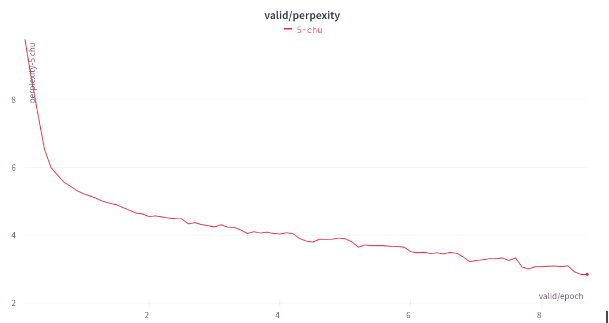
\includegraphics[width=15cm]{Images/21.png} \\[0.25in]

\caption{Perplexity thơ 5 chữ}
\end{center}
\end{figure}
\begin{figure}[h!]
\begin{center}
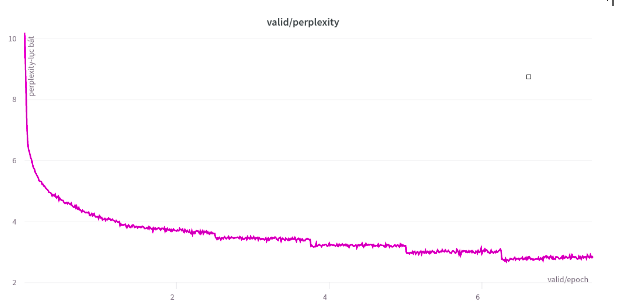
\includegraphics[width=15cm]{Images/22.png} \\[0.25in]

\caption{Perplexity thơ lục bát}
\end{center}
\end{figure}

\newpage
\newpage
\subsection{Tự động đánh giá thơ lục bát}
Thơ lục bát có cách gieo vần đặc biệt so với các thể thơ khác, với thể thơ này ta có các quy luật rõ ràng để gieo:\\
 Gieo Vần-Chữ cuối của câu trên (tức câu 6) phải vần với chữ thứ sáu của câu dưới (tức câu 8). Cứ mỗi hai câu thì đổi vần, & bao giờ cũng gieo vần bằng (còn gọi là bằng hoặc bình, tức có dấu huyền hoặc không dấu). Dựa vào tính chất trên ta có thể tạo ra một từ điển gồm các subword có vần với nhau như hình 23.
\begin{figure}[h!]
\begin{center}
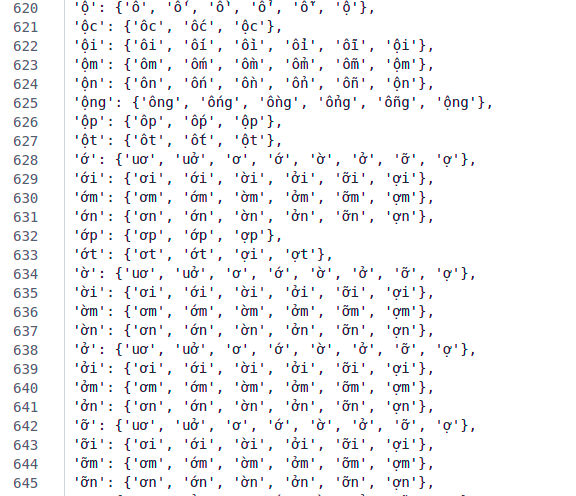
\includegraphics[width=12cm]{24.png} \\[0.15in]

\caption{Từ điển  các vẫn trong tiếng Việt}
\end{center}
\end{figure}
\newpage 
Với từ điển này, ta có thể kiểm tra câu sinh ra có vần với câu đúng quy tắc gieo vần hay không. 

Tương tự với luật bằng trắc:  Luật Bằng Trắc: Luật Bằng Trắc-Cách sử dụng mẫu tự & viết tắt giống như sau: B là Bằng, T là Trắc, V là Vần.
\begin{itemize}
    \item Làm câu lục trước tuân thủ luật thơ ở các tiếng 2,4,6 là B – T -B, các tiếng còn lại tự do
    \item Tiếp đến câu bát: cân chỉnh cho có sự đối xứng ở các tiếng 2, 4, 6 là B – T – B – B, các tiếng còn lại tự do
\end{itemize}
\begin{figure}[h!]
\begin{center}
\includegraphics[width=12cm]{Images/Hình 26.png} \\[0.15in]

\caption{Từ điển các dấu có thể có của các subword}
\end{center}
\end{figure}
Vì thế ta hoàn toàn có thể kiểm tra được câu được sinh ra có đáp ứng quy luật hay không.
Chúng ta có thể dễ dàng xác định rằng có (3 * n-1) từ cần kiểm tra vần và (7 * n) từ có âm trong mỗi khổ thơ, trong đó n là số lượng các cặp câu. Vì vậy ta có thể tạo ra công thức tính điểm với mục tiêu là maximize nó như sau: 
$$\text{Score} = 100*(1-\frac{R}{3n-1} - \frac{T}{7n})$$
Trong đó:
\begin{itemize}
    \item R là số lượng từ có cách gieo vần sai

    \item T là số lượng từ có cách gieo luật bằng trắc sai
\end{itemize}

\textbf{Kết quả cuối cùng} được đánh giá trên 50 bài thơ lục bát với điểm số thu được là \textbf{70.7035}. 
\subsection{Human evaluation}
Cách tốt nhất để đánh giá một bài thơ có đáp ứng đủ về mặt ngữ nghĩa và mặt luật thơ cõ lẽ đánh giá bằng người đọc, người đọc có thể cảm nhận được tính nội dung ngữ nghĩa sinh ra và cách gieo vần một cách khách quan.\\
Qua quá trình sinh thử gần 100 bài thơ ở 4 thể loại (5 chữ, 7 chữ, 8 chữ, lục bát) chúng tôi đem ra kết luận như sau: về mặt nội dung, những chủ đề quen thuộc như gia đinh, tình yêu, quê hương các mô hình sinh ra về mặt ngữ nghĩa và luật tốt, tuy nhiên với những chủ để hiếm gặp như khủng bố, kinh tế, chính trị thì về kết quả thu được vẫn đáp ứng là có vần tuy nhiên về mặt ngữ nghĩa thì nó còn kém. Điều này có thể giải thích vì dữ liệu ở trên những miền đó ít xuất hiện hơn so với miền gia đình, tình yêu, quê hương nên mô hình sinh ra không được tốt bằng.
\newpage
\section{Triển khai ứng dụng}
\subsection{Thiết kế hệ thống }
Mục tiêu: Xây dựng một website để người dùng tương tác, gửi yêu cầu về một bài thơ với từ khóa và thể thơ tương ứng.\\
\begin{figure}[h!]
\begin{center}
\includegraphics[width=12cm]{Images/Hình 27.png} \\[0.2in]

\caption{Thiết kế hệ thống}
\end{center}
\end{figure}
\newline
Tại tầng giao diện, người dùng sẽ nhập từ khóa và chọn thể thơ mong muốn. Sau đó tầng giao diện sẽ gửi yêu cầu về cho tầng máy chủ.\\
Tại tầng máy chủ, model huấn luyện thể thơ tương ứng sẽ được gọi và đưa ra output là bài thơ tương ứng. Tầng máy chủ trả kết quả lại cho tầng giao diện để hiển thị cho người dùng\\

Phía backend sẽ xây dựng một hàm xử lý với input đầu vào là từ khóa và thể thơ nhận được từ phía front-end gửi xuống. Hàm sẽ gọi đến model huấn luyện với từ khóa và thể thơ tương ứng để tiến hành sinh thơ và trả kết quả hiển thị ra cho front-end
\begin{figure}[h!]
\begin{center}
\includegraphics[width=16cm]{Images/Hình 28.png} \\[0.2in]

\caption{Giao diện Web}
\end{center}
\end{figure}
\subsection{Cài đặt}
Để cài đặt chương trình, chúng tôi có 3 cách để cài đặt: 
\begin{enumerate}[Cách 1.]
\item clone code ở link github  https://github.com/dantruonghtno1/Vietnamese-poetry và sau đó run: 
\item clone code ở link github https://github.com/dantruonghtno1/Vietnamese-poetry build docker images từ file Dokerfile để run container 
\item Kéo container từ trên docker hub: https://hub.docker.com/repository/docker/dantruonghtno1/poem  xuống sau đó chỉ cần run conteiner là được.

\end{enumerate}


\newpage






\section{Kết luận}
Với cách tiếp cận đơn giản sử dụng pretrained model GPT-2 để fine tuning trên các bộ dữ lệu thơ 5 chữ, 7 chữ, 8 chữ và thơ lục bát với chú ý khi fine tuning là ta thêm toekn <endline> và bộ từ điển để mô hình của ta học được quy luật xuống dòng. Chúng tôi đã đánh giá trên 3 cách đánh giá (perplexity, đánh giá luật thơ lục bát đối với mô hình sinh thơ lục bát, và human evaluation thấy được rằng việc sinh thơ ở các ngữ cảnh về gìa đình tình yêu, quê hương có xu hướng sinh ra tốt hơn nhưng ngữ cảnh về chính trị, kinh tế, ... Điều này có thể giải thích vì dữ liệu thu thập là những bài thơ chủ yểu viết trên miền gia đình tình yêu, quê hương. \\

Các bài thơ được sinh mẫu được tập hợp lại tại \href{https://docs.google.com/document/d/1sY8Tu338GKSADCaPOD5k6xwEup9CImZg1dTlMnnN8Z8/edit#heading=h.gjrc6wgpnklp}{[]link 1]} và \href{https://drive.google.com/drive/folders/1fHVltUx2b5-7ViffQqSPe07KLlotM-ME}{[]link 2]}
Định hướng tương lai: trong tương lai chúng tôi sẽ tiếp tục phát triển thêm tính năng đối thớ - đầu vào là câu thơ của người dùng, model sẽ học ngữ cảnh đó và sinh ra câu tiếp theo. Và ngoài ra tại hội nghị CoRR 2021 VinAI có công bố một pretrain mới cho tiếng Việt là BARTPho \href{https://arxiv.org/abs/2109.09701}{[19]} với kết quả mà bài báo đăng tải, chúng tôi hi vọng nó sẽ cải thiện chất lượng sinh thơ của ta. 
\newpage
\section{Tư liệu tham khảo}

\begin{enumerate}[ 1.]
\item One the road en.wikipedia.org/wiki/1\_the\_Road
\item Ilya Sutskever, Oriol Vinyals, Quoc V. Le: Sequence to Sequence Learning with Neural Networks https://arxiv.org/abs/1409.3215
\item Vanishing gradient problem en.wikipedia.org/wiki/Vanishing\_gradient\_problem
\item Minh-Thang Luong, Hieu Pham, Christopher D. ManningEffective Approaches to Attention-based Neural Machine Translation https://arxiv.org/pdf/1508.04025.pdf
\item Ashish Vaswani, Noam Shazeer, Niki Parmar, Jakob Uszkoreit, Llion Jones, Aidan N. Gomez, Lukasz Kaiser, Illia Polosukhin Attention Is All You Need https://arxiv.org/abs/1706.03762
\item Lantao Yu, Weinan Zhang, Jun Wang, Yong Yu SeqGAN: Sequence Generative Adversarial Nets with Policy Gradient
\item Yifan Jiang, Shiyu Chang, Zhangyang Wang TransGAN: Two Pure Transformers Can Make One Strong GAN, and That Can Scale Up https://arxiv.org/abs/2102.07074

\item 	Wu, X. Tosa, N. Nakatsu, R. New Hitch Haiku: An interactive Renku poem composition supporting tool applied for sightseeing navigation system https://scholarbank.nus.edu.sg/handle/10635/71127
\item Gaiku : Generating Haiku with Word Associations Norms https://aclanthology.org/W09-2005.pdf
\item PoeTryMe: a versatile platform for poetry generation  \href{https://www.researchgate.net/publication/236445297_PoeTryMe_a_versatile_platform_for_poetry_generation}{ PoeTryMe: a versatile platform for poetry generation }
\item Long Jiang, Ming Zhou Generating Chinese Couplets using a Statistical MT Approach https://aclanthology.org/C08-1048/
\item Generating chinese classical poems with statistical machine translation models https://dl.acm.org/doi/10.5555/2900929.2900962
\item  \href{https://www.semanticscholar.org/paper/Chinese-Poetry-Generation-with-Recurrent-Neural-Zhang-Lapata/229ec55602143271867682d181ec35f2e43e06e8}{Chinese Poetry Generation with Recurrent Neural Networks}
\item Generating chinese classical poems with rnn encoder-decoder https://arxiv.org/pdf/1604.01537.pdf
\item \href{https://d4mucfpksywv.cloudfront.net/better-language-models/language_models_are_unsupervised_multitask_learners.pdf}{GPT2 Language Models are Unsupervised Multitask Learners}
\item  GPT-based Generation for Classical Chinese Poetry https://arxiv.org/abs/1907.00151

\item Deep Residual Learning for Image Recognition https://arxiv.org/abs/1512.03385
\item gpt2-viwiki https://huggingface.co/danghuy1999/gpt2-viwiki
\item perplexity Standford http://web.stanford.edu/class/cs224n/slides/cs224n-2021-lecture05-rnnlm.p
\item SP-GPT2: Semantics Improvement in Vietnamese
Poetry Generation https://arxiv.org/pdf/2110.15723.pdf
\end{enumerate}
\newpage
\section{Phụ lục: Một số bài thơ được sinh}
\subsection{Thơ lục bát}
\textbf{Bài 1}: \\
 chia tay anh ra chiến trường \\
 còn em ở lại hậu phương học nghề \\
 bên bờ sông gió lạnh se \\
 lời anh thủ thỉ em nghe ấm lòng \\
anh ơi mỗi năm mùa đông \\
 sao em quên được tình nồng anh trao \\
xuân về rực thắm mai đào \\
 bên song cửa sổ ước ao gặp chàng\\
\textbf{Bài 2}:\\
mẹ cha về cõi vĩnh hằng \\
 đắng cay chín tháng tiện tằn bước đi \\
  nén nhang lưng nghẹn ướt mi \\
 hương đăng thắp nén bờ mi u buồn \\
chiều tà thư thả bay luôn \\
 nghĩ thương cha mẹ lệ tuôn tuôn trào \\
 con cháu thanh thản tự hào \\
 những lời cha mẹ đặt vào tim con\\
\textbf{Bài 3}: \\
tình yêu như ánh ban mai \\
 long lanh hoa lá đọng vài giọt sương \\
chập chờn ong bướm trong vườn \\
 hoa ru giọt mật dẫn đường tình yêu \\
hàng cây chim đậu hót kêu \\
 con tim réo gọi đâm liều yêu em \\
nghiêng soi em đứng bên thềm \\
 sưởi hong mái tóc điểm thêm hoa cài\\
\subsection{Thơ 8 chữ}
\newline
\textbf{Bài 1}: \\

 đông đã về rồi em có về không \\
 khung trời cũ trải lòng ta sóng gió\\ 
 cả không gian vạn vì sao sáng tỏ \\
 se sắt lòng nhung nhớ sợi tình hoang \\
 phủ hồn ta trên khắp nẻo non ngàn \\
 niềm day dứt vạn lần không còn nữa \\
 nụ ái ân nguyện một đời chọn lựa \\
 ngập men say từng chập một cuộc tình\\


\textbf{Bài 2}:\\
 thương em nhiều tình cách trở hai nơi\\ 
 nhớ em lắm anh gửi vào trong gió \\
 đêm lạnh buồn gió đông về cuối ngõ \\
 hai phương trời vò võ vậy không em \\
 anh gởi em chút hạnh phúc ấm êm \\
 chút kỉ niệm êm đềm trên giấy trắng \\ 
 chút tình ấm chút say nồng sâu lắng \\
 em gửi tình chút bối rối hờn ghen\\

\textbf{Bài 3}: \\
buồn vô cớ khóc hoài trong lặng lẽ \\
 trong âm thầm khe khẽ gọi tên ai \\
 suốt năm tháng cô đơn hoài quạnh quẽ\\ 
 trách than đời đã lỡ chuyến đò ngang \\
 phận số hẩm đời không xanh sắc lá \\
 kiếp hồng trần anh đã có em rồi \\
 yêu em lắm làm sao mà ích kỷ \\
 để kiếp người phải sống cảnh đơn côi\\
\subsection{Thơ 7 chữ}
\textbf{Bài 1}\\
yêu nhau thắm thiết áng thơ xinh \\
 cách trở xa xôi kết nghĩa mình \\
 duyên phận ngàn năm đời luyến nhớ \\
 trăng sương vạn chuỗi ánh rung rinh \\
 mộng lòng say đắm hồn phu phụ \\
 chăn gối yêu thương bóng bạn tình \\
 năm tháng vấn vương niềm ước vọng \\
 thuyền duyên lướt sóng ánh lung linh\\
 \\
\textbf{Bài 2}\\
 yêu thương sâu đậm lắm chi li \\
 lo lắng bận lòng mỗi bước đi \\
 gần gũi ngọt ngào trao thủ thỉ \\
 trái ngang da diết gửi rù rì \\
 hương đưa khoảnh khắc hồn lưu niệm \\
 chim hót một lần dạ khắc ghi \\
 xa vắng u hoài treo suối biếc \\
 bâng khuâng thao thức nhỏ sầu bi\\
\subsection{Thơ 5 chữ}
\textbf{Bài 1}:\\
 yêu em từ trong nôi \\
 yêu em chưa biết ngồi \\
 yêu em những ngây dại \\
 yêu em hồn trắng trong \\
 yêu em thời con gái \\
 hồn nhiên mái tóc dài \\
 tương tư đêm nằm ngủ \\
 gửi tình trong giấc mơ\\
\textbf{Bài 2}: \\
 tình yêu là dòng sông \\
 khi trời mây oi nồng \\
 ta ngâm mình trong đó \\
 nghe dịu mát nơi lòng \\
 tình yêu trong hy sinh \\
 luôn quên bản thân mình\\ 
 niềm tin đan thương nhớ \\
 cành duyên nở hoa xinh\\
\textbf{Bài 3}:\\
 mẹ ơi con rất sợ \\
 mỗi khi mùa xuân về \\
 tóc mẹ lại thêm bạc \\
 lưng mẹ cũng thêm còng \\
 mẹ ơi con rất sợ \\
 mỗi năm mùa xuân về \\
 mẹ ngồi ngóng con trẻ \\
 có đứa nào về chưa\\

\end{document}

